\documentclass[10pt,twoside, fleqn]{memoir}
%\usepackage{createspace}
%\usepackage[size=pocket,noicc]{createspace}
%\usepackage[paperwidth=4.25in, paperght=6.875in,bindingoffset=.75in]{geometry}
\usepackage[T1]{fontenc}
\usepackage{mathpazo} % USE PALATINO FONT
%\usepackage{newpxtext,newpxmath}
\usepackage[latin1]{inputenc}
\usepackage[xindy]{imakeidx}
\usepackage[nomain,acronym,xindy,toc]{glossaries}
%\usepackage{glossaries} %For acronyms
\usepackage[british]{babel}
%\usepackage{tgtermes}
%\usepackage[framed, numbered, autolinebreaks]{mcode} %MATLAB Snippet code
\usepackage{listings}
\usepackage{graphicx}

%\usepackage{hyperref} % HYPERLINKS
\usepackage[font=footnotesize]{caption}
\usepackage{subcaption}
\usepackage{pdflscape} %Landscape pages
\usepackage{pdfpages}
\usepackage{amsmath}
\usepackage{amssymb}
\usepackage{gensymb} %Degree sign
\usepackage{footnote} %Footnotes in tabulars
\usepackage{xcolor,framed,marginnote,blindtext}
\usepackage{listings} %Include code

%\usepackage{vrsion}
\colorlet{shadecolor}{blue!10}
%\usepackage[fleqn]{amsmath}


\usepackage{tikz} %TO CREATE BLOCK DIAGRAMS
\usetikzlibrary{shapes,arrows}
\usetikzlibrary{positioning}

\setcounter{tocdepth}{2} % DEPTH OF TABLE OF CONTENTS; 2= SUBSECTIONS INCLUDED
\setcounter{secnumdepth}{2} % SUBSECTIONS ARE NUMBERED

\usetikzlibrary{positioning}


%\usepackage{mathpazo}
%\usepackage[protrusion=true,expansion=true]{microtype}
%\usepackage{type1cm}
%\usepackage{lettrine}

%\checkandfixthelayout

% See the ``Memoir customise'' template for some common customisations
% Don't forget to read the Memoir manual: memman.pdf

%\title{TITLE OF BOOK}
%\author{NAME OF AUTHOR}
%\date{} % Delete this line to display the current date

%% BEGIN TITLE

\makeatletter
\def\maketitle{%
  \null
  \thispagestyle{empty}%
  \vfill
  \begin{center}\leavevmode
    \normalfont
    {\LARGE\raggedleft \@author\par}%
    \hrulefill\par
    {\huge\raggedright \@title\par}%
    \vskip 1cm
  {\Large \@date\par}%
  \end{center}%
  \vfill
  \null
  \cleardoublepage
  }
\makeatother
\author{Paolo Baesso}
\title{Proto DUNE board: pc053a.}
\date{\today}
%\date{23 February 2015}


\input{O:/LatexFiles/Glossary/myGlossary.tex}
\makeglossaries

%%% BEGIN DOCUMENT
\makeindex
\begin{document}

\let\cleardoublepage\clearpage


\maketitle
\frontmatter

\null\vfill
\begin{flushleft}
\textit{Board pc053a.}\newline
\newline
Paolo Baesso - 2016\newline paolo.baesso@bristol.ac.uk
\bigskip

\end{flushleft}
\let\cleardoublepage\clearpage

\newpage
\tableofcontents

\mainmatter
\sloppy

\newenvironment{SpecialPar}
  {\begin{shaded}\noindent}
  {\end{shaded}}



%%% INCLUDE CHAPTERS
\def\brd{pc052a}
%\include{ch_Introduction}
\noindent SFP: optical serial interface.\\
MASTER: RJ45 interface. Can do serial and parallel.\\
SLAVE: RJ45 interface. Can only do parallel.\\

\include{ch_I2C}

\begin{figure}[h]
  \centering
  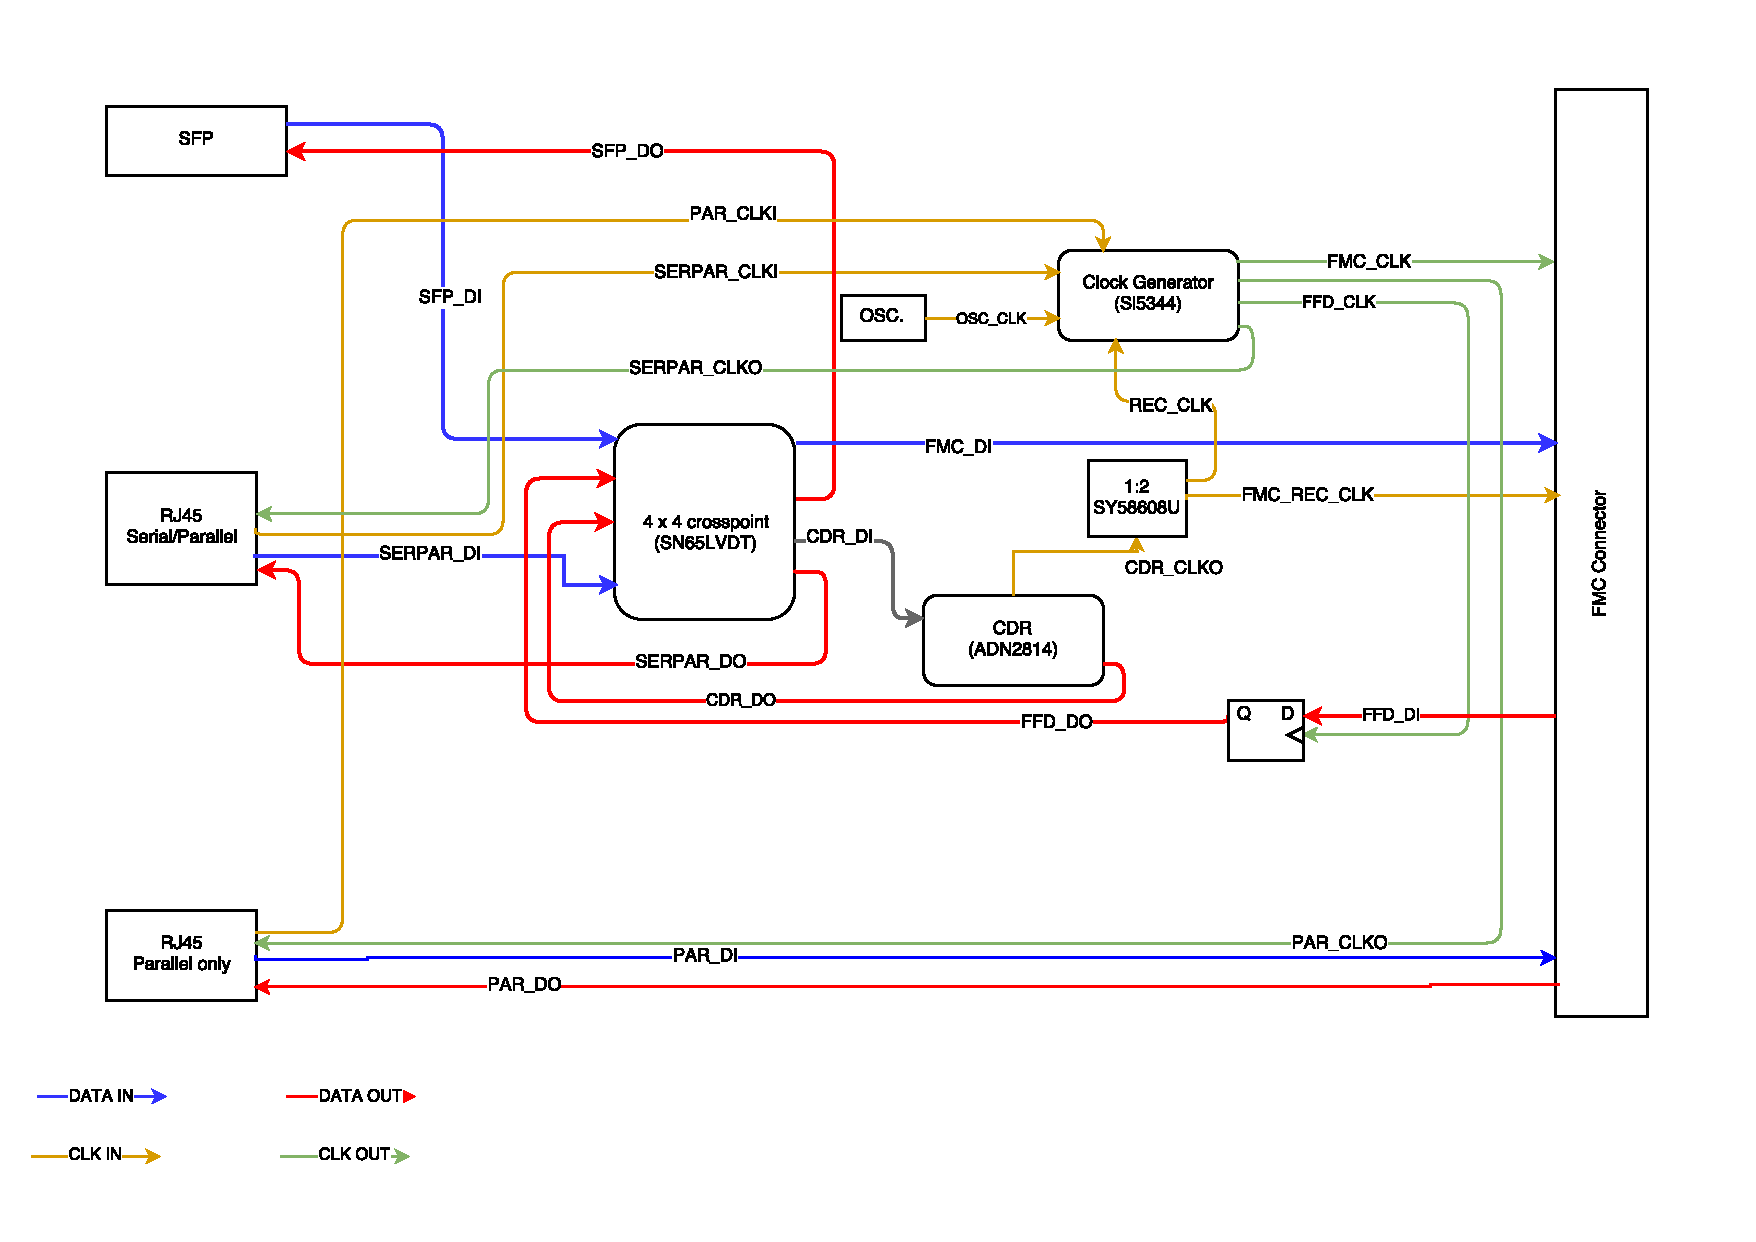
\includegraphics[width=1.62\textwidth, angle=90]{./Images/protoDUNE_fmc_sfp_to_slave_v0-7.pdf}
  \caption{Sketch of the connections and signal names between the elements of the board.}\label{fig:Connections}
\end{figure}

\section{Schematic}
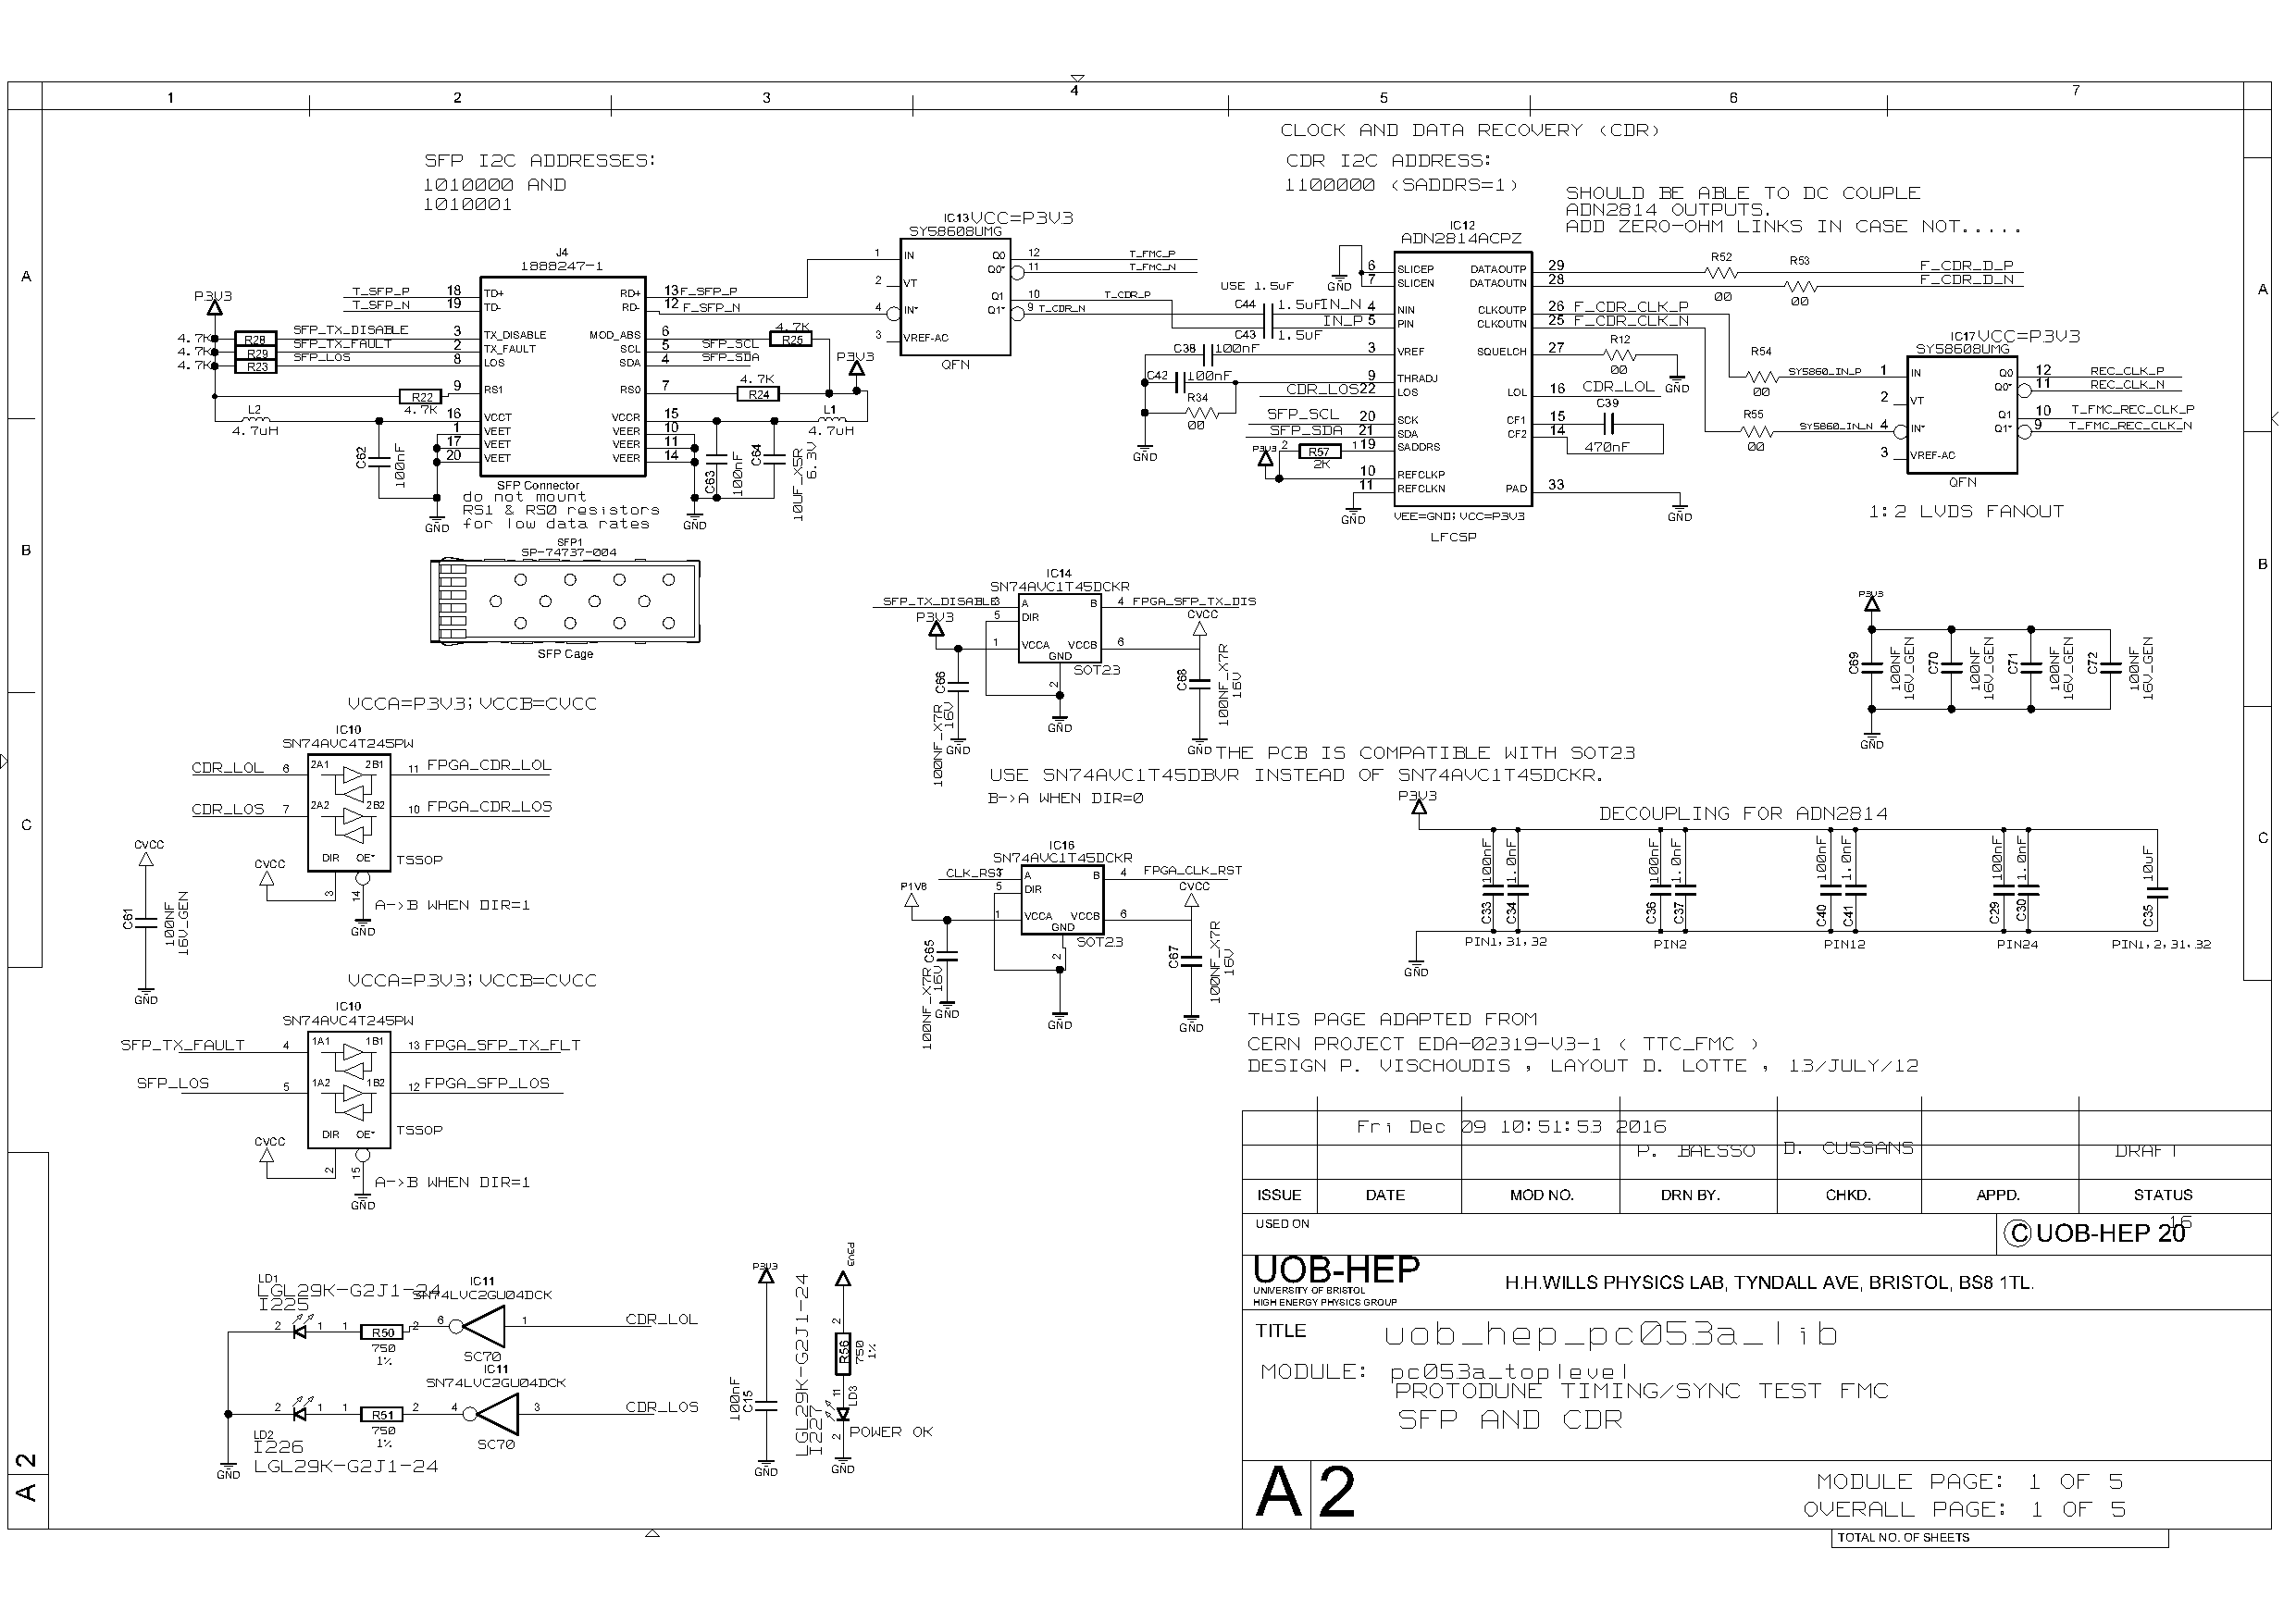
\includepdf[pages={1-},scale=0.99, landscape=true]{./Images/PC053A.pdf}
%\includepdf[pages={1-},scale=0.99, landscape=true]{./Images/PC053A_TOPLEVEL.pdf}


%%% GLOSSARY
\printglossaries
%\printglossary[type=\acronymtype]
\printglossary[type=\acronymtype,title=Abbreviations]

%%% BIBLIOGRAPHY
%\bibliographystyle{unsrt}
%\bibliography{./../../Bibliography/myBibliography}


\end{document} 